\documentclass[a4j,11pt]{ltjsarticle}    % 文章クラスとオプション設定
%%%%%%%%%% スタイル %%%%%%%%%%%%%%%%%%%%%%%%%%%%%%%%%%%%%%%%%%%%%%%%%%%%%%%%%%%%%%%%%%%%%%%%%%%%%%

\usepackage{comment}    % 複数行コメント

% 余白の調整
\usepackage[top=30truemm,bottom=30truemm,left=20truemm,right=20truemm]{geometry}

% 数式関連
\usepackage{amsmath,amssymb,nccmath}    % 数式
\usepackage{bm}         % ベクトルの太文字
\newcommand{\alignref}[1]{\textbf{式(\ref{#1})}}    % 数式参照
\usepackage{siunitx}

% 画像関連
\usepackage{pdfpages} % PDF
\usepackage{graphicx} % 画像

\usepackage{here}% figureの位置調整
% 表設定
\usepackage{multirow}   % 表の行の結合
\usepackage{longtable}  % ページをまたぐ長い表
\renewcommand{\tablename}{\textbf{Table.}}   % 表キャプション
\newcommand{\tablenameref}[1]{\textbf{Table.\ref{#1}}}  % 表の参照を定義

\usepackage{tikz} %図を描く
\usetikzlibrary{positioning, intersections, calc, arrows.meta,math} %tikzのlibrary

%%%%%%%%%% 本文 %%%%%%%%%%%%%%%%%%%%%%%%%%%%%%%%%%%%%%%%%%%%%%%%%%%%%%%%%%%%%%%%%%%%%%%%%%%%%%%%%

\begin{document}

% % !TEX root = main.tex

%%%%%%%%%%%%%%%%%%%%%%%%%%%%%%%%%%%%%%%%%%%%%%%%%%%%%%%%%%%%%%%%%%%%%%%%%%%%%%%%%%%%%%%%%%%%%%%%

\title{タイトル}
\author{氏名\thanks{所属}}
\date{年月日}
\maketitle

%%%%%%%%%%%%%%%%%%%%%%%%%%%%%%%%%%%%%%%%%%%%%%%%%%%%%%%%%%%%%%%%%%%%%%%%%%%%%%%%%%%%%%%%%%%%%%%%

% \setcounter{tocdepth}{3}
% \tableofcontents
% \newpage

\subsection*{問題1}
電子回路によく使われるコンデンサには,電解コンデンサとセラミックコンデン
サがある.両者の周波数特性とその用途を調べよ.
\begin{description}
    \item[] 電解コンデンサとセラミックコンデンサの周波数特性は図1に示す.また,
    電解コンデンサとセラミックコンデンサの用途は以下のとおりである.
    \begin{itemize}
        \item 電解コンデンサの用途
        \begin{description}
            \item[] 平滑用,デカップリング用
        \end{description}
        \item セラミックコンデンサの用途
        \begin{description}
            \item[] 平滑用,カップリング用,デカップリング用,高周波回路
        \end{description}
    \end{itemize}
\end{description}

\begin{figure}[H]
    \centering
    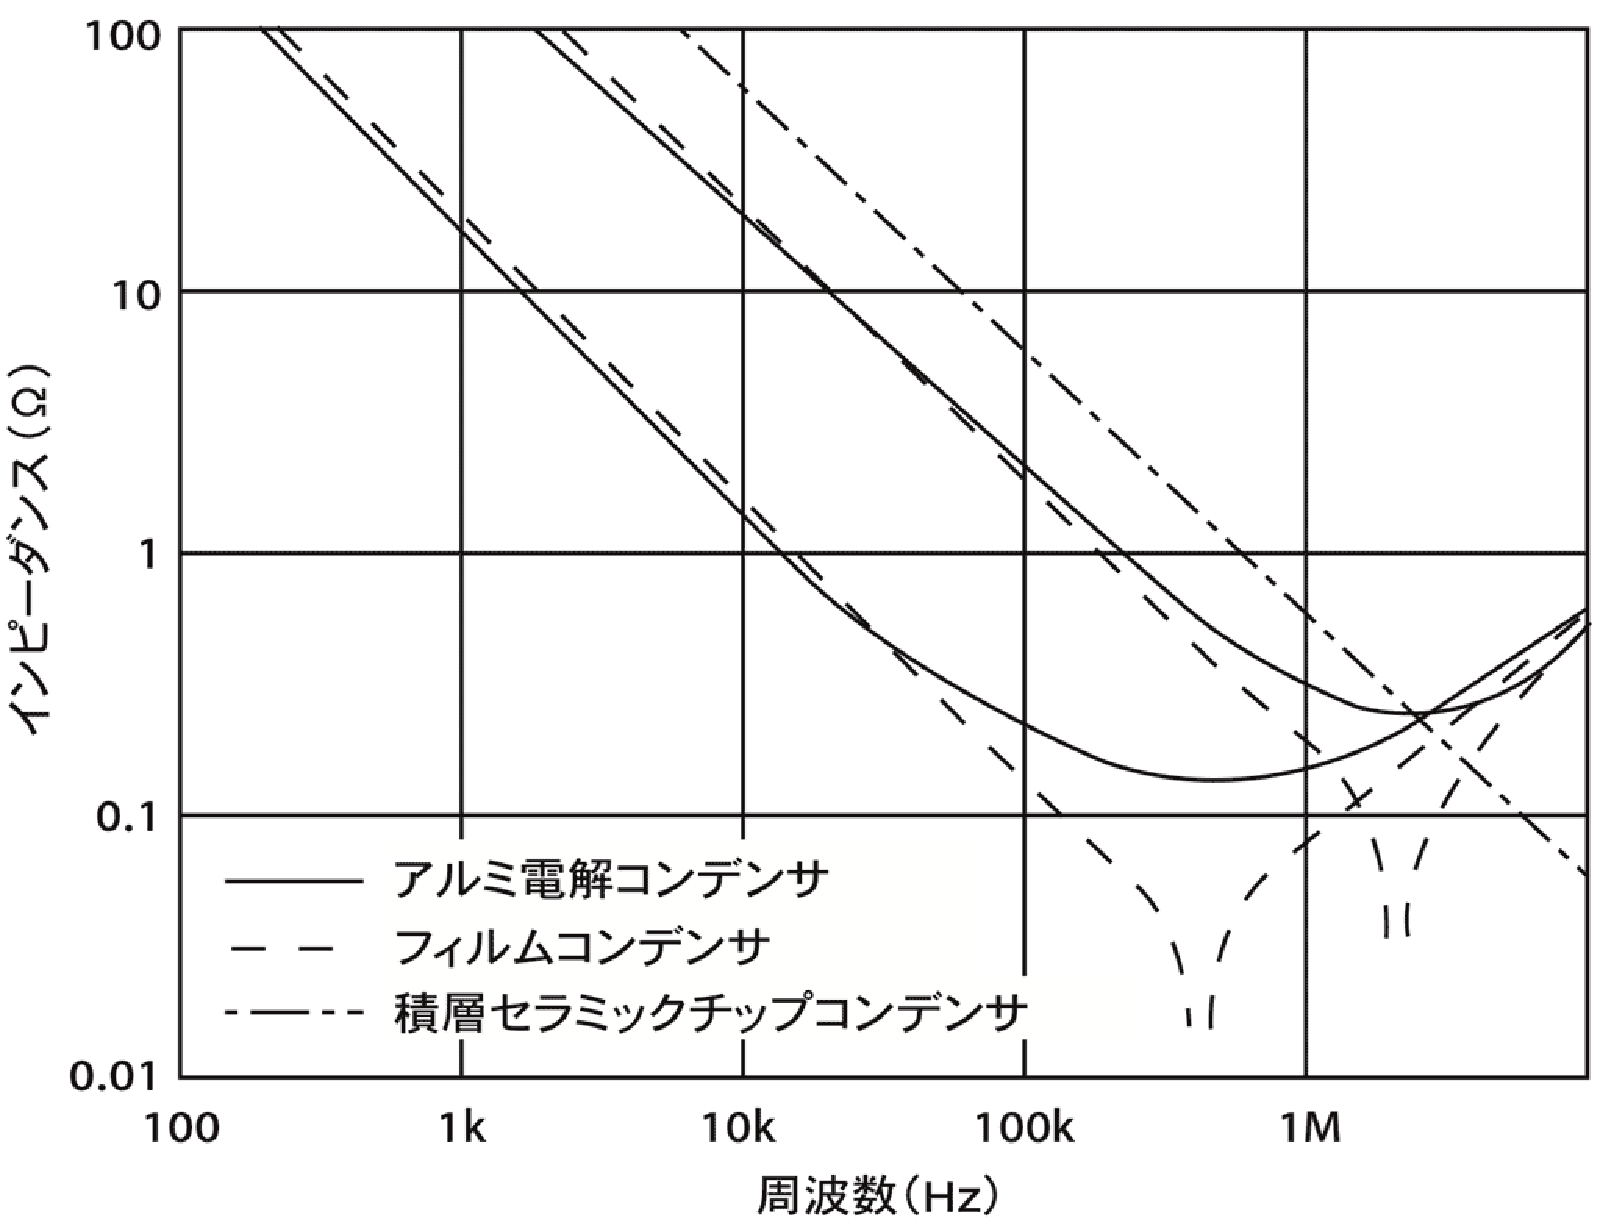
\includegraphics[scale=0.4]{figure1.pdf}
    \caption{電解コンデンサとセラミックコンデンサの周波数特性}
\end{figure}

\subsection*{問題2}
ダイオードの逆方向降伏電圧を用いて一定の電圧を発生するダイオードをな
んと呼ぶか?
\begin{description}
    \item[] ツェナーダイオード
\end{description}

\subsection*{問題3}
LEDには,赤,青,緑等に発光するものがある.色の違いが何によるのか,
青色ダイオードはなぜ最後に発明されたのかを考察せよ.
\begin{itemize}
    \item LEDの色の違いの原因
    \begin{description}
        \item[] 光の波長の違いが,LEDの発光色を決めており,$450\si{nm}$前後が青色,
        $520\si{cm}$前後が緑色,$660\si{nm}$前後が赤色に見える.さらに,
        この光の波長は,Ga(ガリウム),N(窒素),In(インジウム),Al(アルミニウム)
        ,P(リン)など,LEDの半導体を構成する化合物によって決まる.

    \end{description}
    \item 青色ダイオードが最後に開発された原因
    \begin{description}
        \item[] 青色ダイオードの材料となる化合物半導体,窒素ガリウムとサファイアの原子の間隔の差が大きく、
        きれいな結晶を作るのが難しかったためである.結晶の作成に成功した後も,
        ホールを生み出すマグネシウムに,水素原子がくっついて邪魔をしていたために,
        p型のホールがうまく動かなかったために青色ダイオードの発明が難航した.
    \end{description}
\end{itemize}

% !TEX root = main.tex

%%%%%%%%%%%%%%%%%%%%%%%%%%%%%%%%%%%%%%%%%%%%%%%%%%%%%%%%%%%%%%%%%%%%%%%%%%%%%%%%%%%%%%%%%%%%%%%%
\section{理論}
%%%%%%%%%%%%%%%%%%%%%%%%%%%%%%%%%%%%%%%%%%%%%%%%%%%%%%%%%%%%%%%%%%%%%%%%%%%%%%%%%%%%%%%%%%%%%%%%
図1に示す2つの端子対からなる回路を考える.入力端子対$1,1'$の電圧,電流$V_1$,$I_1$は,
出力端子対$2,2'$の電圧,電流$V_2$,$I_2$により
$$
\left[\begin{array}{c}
V_1 \\
I_1
\end{array}\right]=\left[\begin{array}{ll}
A & B \\
C & D
\end{array}\right]\left[\begin{array}{c}
V_2 \\
I_2
\end{array}\right]
$$
と表される.この式中の2行2列の行列
$$
\left[\begin{array}{ll}A & B \\ C & D\end{array}\right]
$$
をF行列とよび,この行列の各要素$A,B,C,D$を4端子定数とよぶ.4端子定数$A$は出力端子対$2,2'$を開放した時の入力電圧$V_1$と出力電圧$V_2$の比
$$
A=\left.\frac{V_1}{V_2}\right|_{I_2=0}
$$
と定義される.また,$B$は出力端子対$2,2'$を短絡した時の入力電圧$V_1$と出力電流$I_2$の比
$$
B=\left.\frac{V_1}{I_2}\right|_{V_2=0}
$$
であり,$C$は出力端子対$2,2'$を開放した時の入力電流$I_1$と出力電圧$V_2$の比
$$
C=\left.\frac{I_1}{V_2}\right|_{I_2=0}
$$
であり,$D$は出力端子対$2,2'$を短絡した時の入力電流$I_1$と出力電流$I_2$の比
$$
D=\left.\frac{I_1}{I_2}\right|_{V_2=0}
$$
である.


図2のように2端子対回路を縦続接続すると,全体の回路のF行列は各々の回路のF行列の積で表される.
すなわち

$$
\left[\begin{array}{l}
V_1 \\
I_1
\end{array}\right]=\left[\begin{array}{ll}
A & B \\
C & D
\end{array}\right]\left[\begin{array}{c}
V_3 \\
I_3
\end{array}\right]
$$

とすると、

$$
\left[\begin{array}{l}
V_1 \\
I_1
\end{array}\right]=\left[\begin{array}{ll}
A_1 & B_1 \\
C_1 & D_1
\end{array}\right]\left[\begin{array}{l}
V_2 \\
I_2
\end{array}\right]
$$

$$
\left[\begin{array}{c}
V_2 \\
I_2
\end{array}\right]=\left[\begin{array}{ll}
A_2 & B_2 \\
C_2 & D_2
\end{array}\right]\left[\begin{array}{l}
V_3 \\
I_3
\end{array}\right]
$$

より

$$
\left[\begin{array}{ll}
A & B \\
C & D
\end{array}\right]=\left[\begin{array}{ll}
A_1 & B_1 \\
C_1 & D_1
\end{array}\right]\left[\begin{array}{ll}
A_2 & B_2 \\
C_2 & D_2
\end{array}\right]
$$

と表される.


$R,L,C,M$以外の素子を含まない回路では,F行列の行列式$AD-BC$の値は1となる.
また,入力端子と出力端子を入れ替えた回路のF行列は,AとDを入れ替えたものとなる.
% !TEX root = main.tex

%%%%%%%%%%%%%%%%%%%%%%%%%%%%%%%%%%%%%%%%%%%%%%%%%%%%%%%%%%%%%%%%%%%%%%%%%%%%%%%%%%%%%%%%%%%%%%%%
\section{測定}
%%%%%%%%%%%%%%%%%%%%%%%%%%%%%%%%%%%%%%%%%%%%%%%%%%%%%%%%%%%%%%%%%%%%%%%%%%%%%%%%%%%%%%%%%%%%%%%%

\subsection*{測定機器}
コイル,キャパシタ,固定抵抗,ブレッドボード,オシロスコープ,発振器,配線材料,関数電卓,ノートPC

\subsection*{測定手順}
\subsubsection*{理論値計算}
指定された$L,C,R$の値をもとにインピーダンスの理論値を$f = 100$\,[Hz]\sim 100\,[kHz]
の範囲で回路シミュレータを用いて計算し,インピーダンスの大きさ,偏角,電流相対比の
理論曲線をそれぞれ両対数・片対数・通常方眼グラフ用紙にプロットする.
なお,理論値計算では一律にコイルの巻線抵抗を$r_L = 0.6$\,[\Omega]に設定すること.
共振周波数$f_0$\,[Hz],同調度計算のための$f_L,f_H$\,[Hz]は回路シミュレータから
数値的に求めておく.電流相対比のグラフは$f_L,f_H$を含むよう適切に計算帯域を設定せよ.

\subsubsection*{回路}
測定においては,共振回路全体を流れる電流$I$を測定するために測定用の抵抗$R^{\prime}$を直列に
挿入し,図2に示す回路構成をとる.

\subsubsection*{測定1}
発振器から正弦波を発生させ,適当な$R^{\prime}$を用いて図のc点を電圧測定の基準として
$A-c$間$v_1(t)$\,[V]をオシロスコープのCH1,$B-c$間$v_2(t)$\,[V]をCH2で測定する.
回路を流れる瞬間電流値$i(t)$は$i(t)= -v_2 (t)/R^{\prime}$で求まるが,波形が反転している
ことに注意すること.一つの測定周波数$f$\,[Hz]についての測定対象は,
瞬間電圧$v1(t)$と$v2(t)$の最大振幅,周期$f$\,[Hz],$v1(t)$と$v2(t)$の対応する零交差点の
時間幅$ΔT$\,[sec]である.前者二つの振幅値からインピーダンスの大きさを求める.
後者二つの時間幅からインピーダンスの偏角を求める.周波数fはオシロスコープの測定機能を
利用する.測定範囲内で適切に測定し,インピーダンスの周波数特性,電流相対比をそれぞれ
理論値をプロットしたグラフ用紙に記入する.なお,実際の共振周波数$f_0$と$f_L,f_H$を求める
ため,$f_0,f_L,f_H$近傍は詳しく測定すること.

\subsubsection*{使用機器}
\begin{enumerate}
    \item RC発信機(ケンウッド\quad AG-203A)
    \item DSO(Tektronix\quad TBS1022)
    \item ブレッドボード
    \item Qucs\quad 0.0.16
\end{enumerate}
\newpage
% !TEX root = main.tex

%%%%%%%%%%%%%%%%%%%%%%%%%%%%%%%%%%%%%%%%%%%%%%%%%%%%%%%%%%%%%%%%%%%%%%%%%%%%%%%%%%%%%%%%%%%%%%%%
\section{結果}
%%%%%%%%%%%%%%%%%%%%%%%%%%%%%%%%%%%%%%%%%%%%%%%%%%%%%%%%%%%%%%%%%%%%%%%%%%%%%%%%%%%%%%%%%%%%%%%%

\subsection{実験課題1}
ソレノイド底面を$z=0\,[\si{cm}]$とし,各$z$座標における測定結果を以下の
図5~図25に示す.また,$z$座標と磁気プローブの出力$V_{co}$の積分である
$\int_{0}^{t}V_{co}(t)dt$との測定結果を表1に示す.
ただし,磁気プローブの出力$V_{co}$の積分はオシロスコープから得られるデジタルデータ
(テキストデータ)を使用して算出する方法を用いる.

\begin{figure}[H]
    \centering
    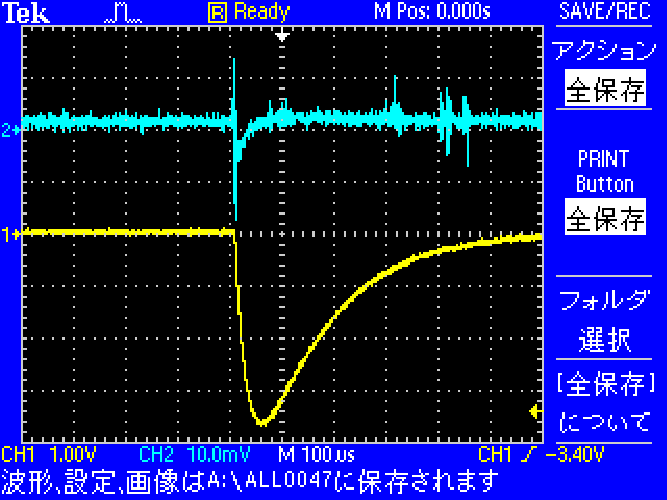
\includegraphics[scale=0.5]{images-22.pdf}
    \caption{$z=-8\,[cm]$における測定結果}
\end{figure}

\begin{figure}[H]
    \centering
    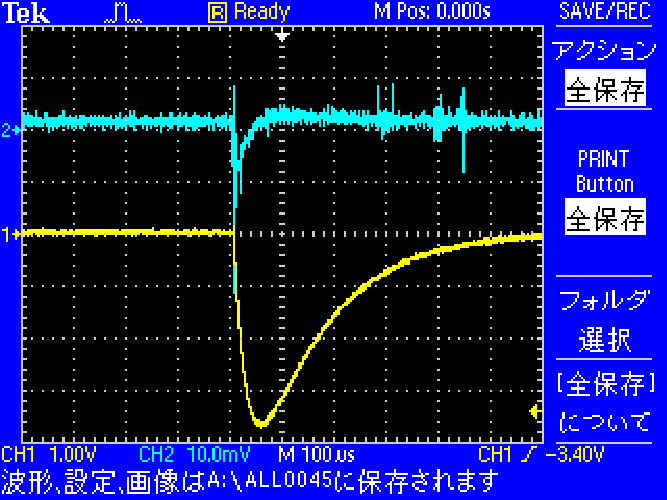
\includegraphics[scale=0.5]{images-21.pdf}
    \caption{$z=-6\,[cm]$における測定結果}
\end{figure}

\begin{figure}[H]
    \centering
    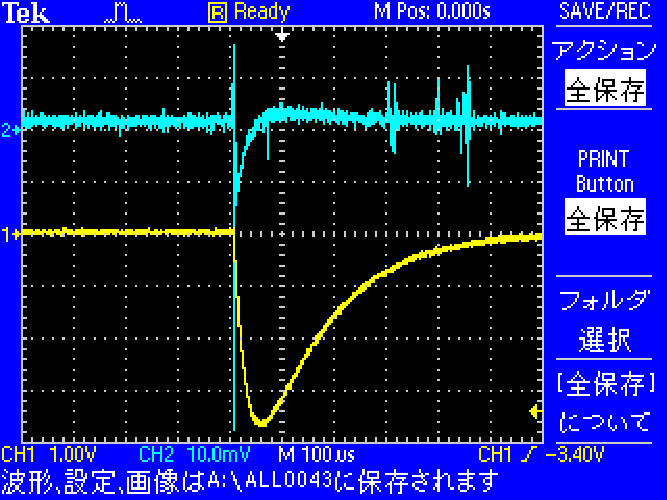
\includegraphics[scale=0.5]{images-20.pdf}
    \caption{$z=-4\,[cm]$における測定結果}
\end{figure}

\begin{figure}[H]
    \centering
    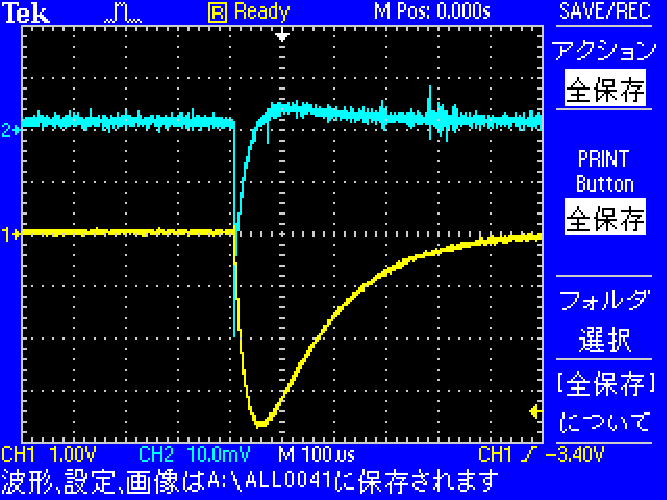
\includegraphics[scale=0.5]{images-19.pdf}
    \caption{$z=-2\,[cm]$における測定結果}
\end{figure}

\begin{figure}[H]
    \centering
    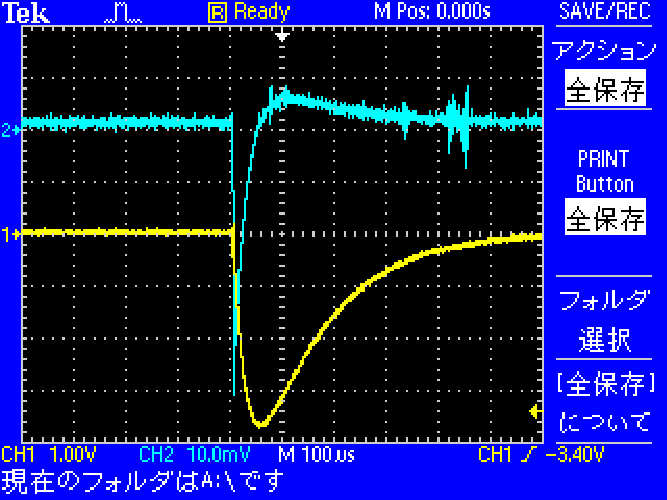
\includegraphics[scale=0.5]{images-1.pdf}
    \caption{$z=0\,[cm]$における測定結果}
\end{figure}

\begin{figure}[H]
    \centering
    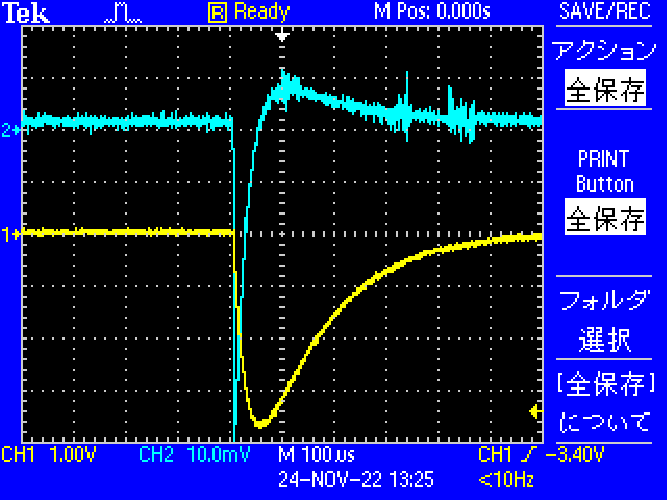
\includegraphics[scale=0.5]{images-2.pdf}
    \caption{$z=2\,[cm]$における測定結果}
\end{figure}

\begin{figure}[H]
    \centering
    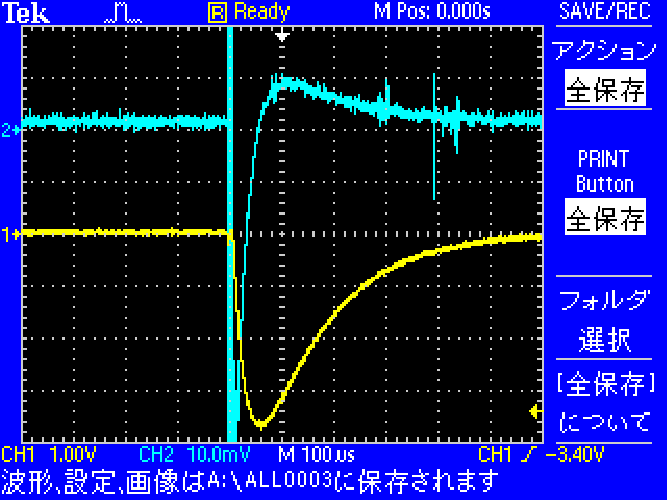
\includegraphics[scale=0.5]{images-3.pdf}
    \caption{$z=4\,[cm]$における測定結果}
\end{figure}

\begin{figure}[H]
    \centering
    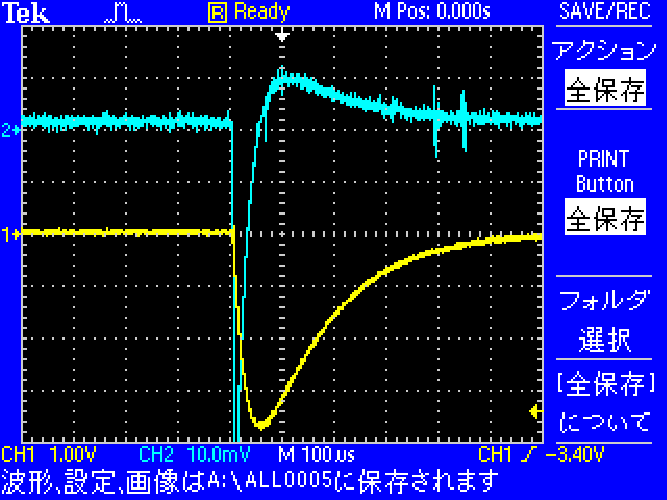
\includegraphics[scale=0.5]{images-4.pdf}
    \caption{$z=6\,[cm]$における測定結果}
\end{figure}

\begin{figure}[H]
    \centering
    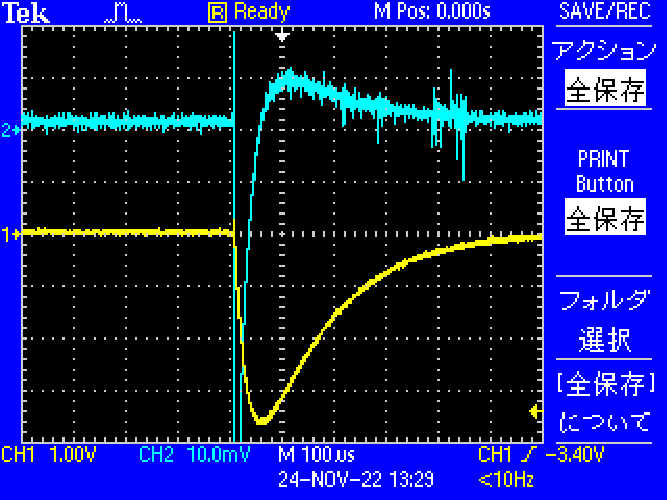
\includegraphics[scale=0.5]{images-5.pdf}
    \caption{$z=8\,[cm]$における測定結果}
\end{figure}

\begin{figure}[H]
    \centering
    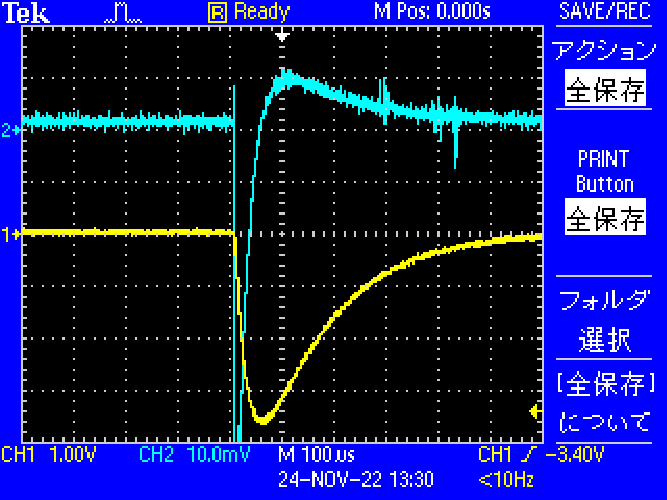
\includegraphics[scale=0.5]{images-6.pdf}
    \caption{$z=10\,[cm]$における測定結果}
\end{figure}

\begin{figure}[H]
    \centering
    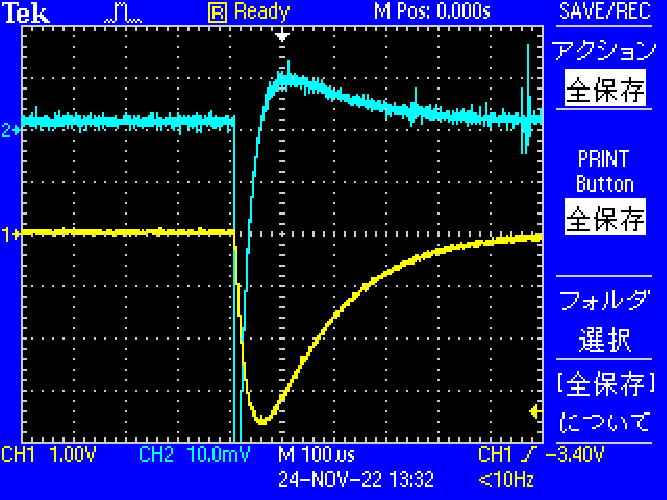
\includegraphics[scale=0.5]{images-7.pdf}
    \caption{$z=12\,[cm]$における測定結果}
\end{figure}

\begin{figure}[H]
    \centering
    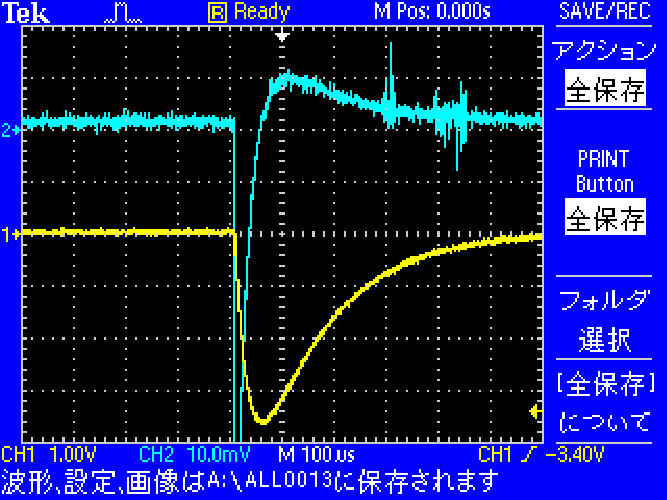
\includegraphics[scale=0.5]{images-8.pdf}
    \caption{$z=14\,[cm]$における測定結果}
\end{figure}

\begin{figure}[H]
    \centering
    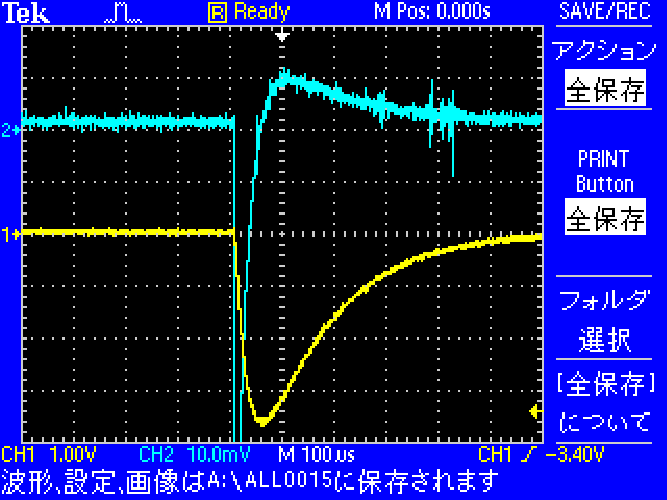
\includegraphics[scale=0.5]{images-9.pdf}
    \caption{$z=16\,[cm]$における測定結果}
\end{figure}

\begin{figure}[H]
    \centering
    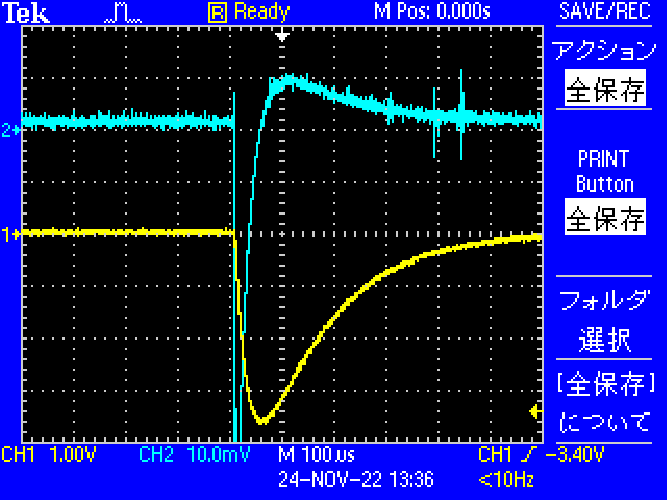
\includegraphics[scale=0.5]{images-10.pdf}
    \caption{$z=18\,[cm]$における測定結果}
\end{figure}

\begin{figure}[H]
    \centering
    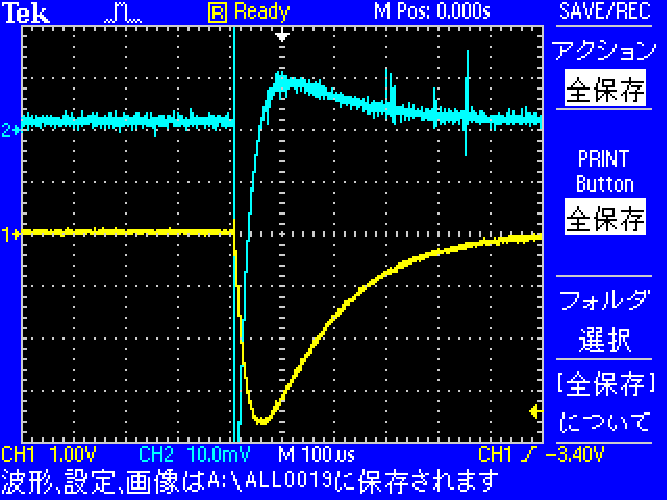
\includegraphics[scale=0.5]{images-11.pdf}
    \caption{$z=20\,[cm]$における測定結果}
\end{figure}

\begin{figure}[H]
    \centering
    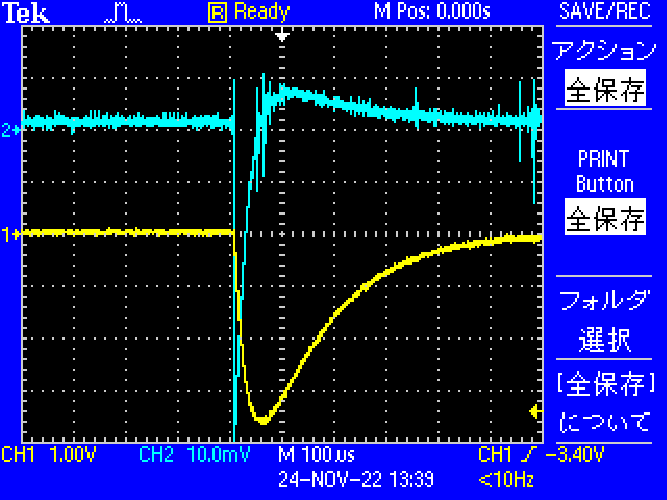
\includegraphics[scale=0.5]{images-12.pdf}
    \caption{$z=22\,[cm]$における測定結果}
\end{figure}

\begin{figure}[H]
    \centering
    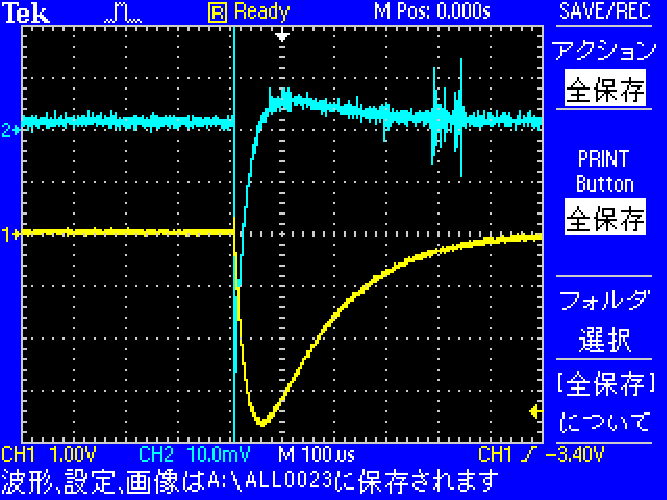
\includegraphics[scale=0.5]{images-13.pdf}
    \caption{$z=24\,[cm]$における測定結果}
\end{figure}

\begin{figure}[H]
    \centering
    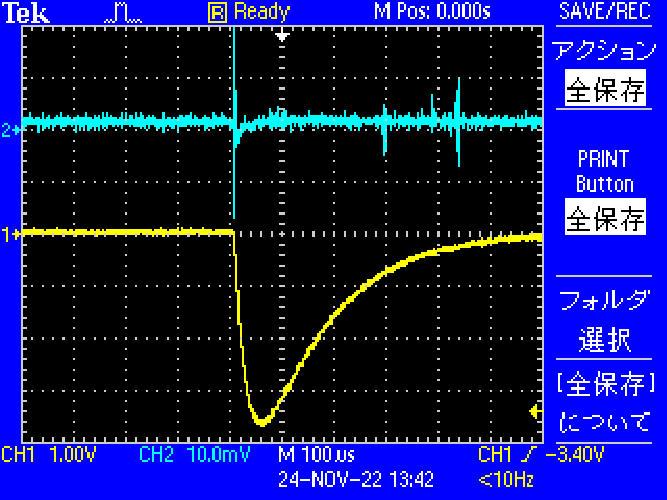
\includegraphics[scale=0.5]{images-14.pdf}
    \caption{$z=26\,[cm]$における測定結果}
\end{figure}

\begin{figure}[H]
    \centering
    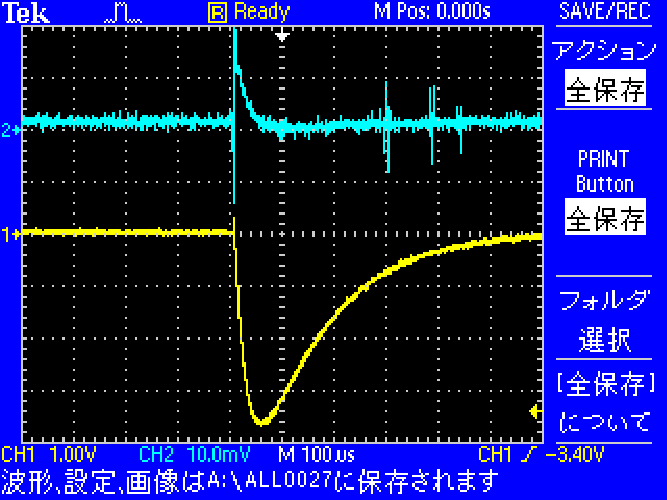
\includegraphics[scale=0.5]{images-15.pdf}
    \caption{$z=28\,[cm]$における測定結果}
\end{figure}

\begin{figure}[H]
    \centering
    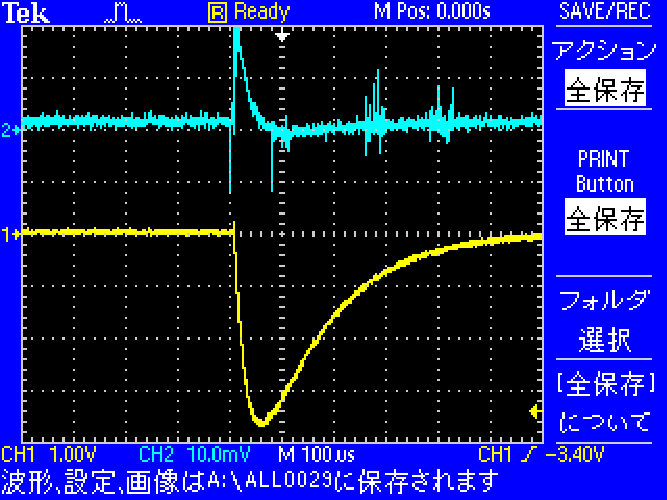
\includegraphics[scale=0.5]{images-16.pdf}
    \caption{$z=30\,[cm]$における測定結果}
\end{figure}

\begin{figure}[H]
    \centering
    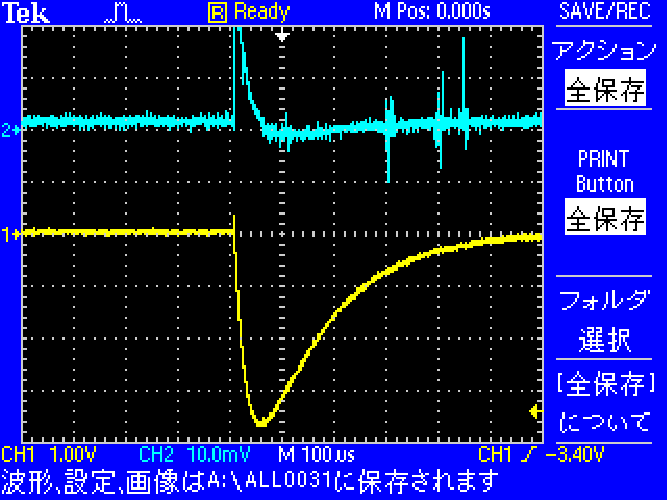
\includegraphics[scale=0.5]{images-17.pdf}
    \caption{$z=32\,[cm]$における測定結果}
\end{figure}

\begin{table}[H]
    \centering
    \caption{磁気プローブの出力$V_{co}$の積分結果}
    \begin{tabular}{c|c}
    \hline
        $z座標\,[\si{cm}]$ & $\int_{0}^{t}V_{co}(t)dt\,[\si{\mu\volt}]$ \\ \hline
        -8 & 0.0706 \\ 
        -6 & 0.154 \\ 
        -4 & 0.221 \\ 
        -2 & 0.421 \\ 
        0 & 0.794 \\ 
        2 & 1.14 \\ 
        4 & 1.40 \\ 
        6 & 1.46 \\ 
        8 & 1.47 \\ 
        10 & 1.49 \\ 
        12 & 1.51 \\ 
        14 & 1.51 \\ 
        16 & 1.49 \\ 
        18 & 1.46 \\ 
        20 & 1.39 \\ 
        22 & 1.04 \\ 
        24 & 0.768 \\ 
        26 & 0.394 \\ 
        28 & 0.336 \\ 
        30 & 0.511 \\ 
        32 & 0.591 \\ \hline
    \end{tabular}
\end{table}

\newpage

\subsection{実験課題2}
鎖交数を変化させた際の,各鎖交数における測定結果を図26~図30に示す.
また,鎖交数と,抵抗$R$の両端の電圧波形$V_R$のピーク電圧$V_{Rmax}$と,
ロゴスキーコイルの出力$V_e$の積分である$\int_{0}^{t}V_e(t)dt$
との測定結果を表2に示す.ただし,ロゴスキーコイルの出力$V_e$の積分は
オシロスコープから得られるデジタルデータ
(テキストデータ)を使用して算出する方法を用いる.

\begin{figure}[H]
    \centering
    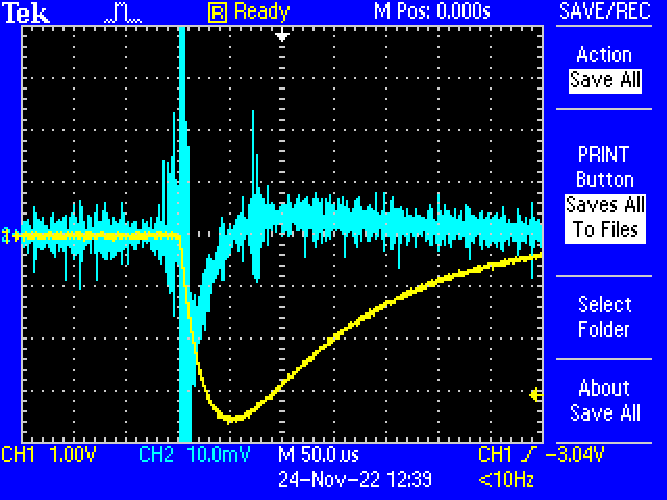
\includegraphics[scale=0.5]{rogowskii-1.pdf}
    \caption{鎖交数が1の時の測定結果}
\end{figure}

\begin{figure}[H]
    \centering
    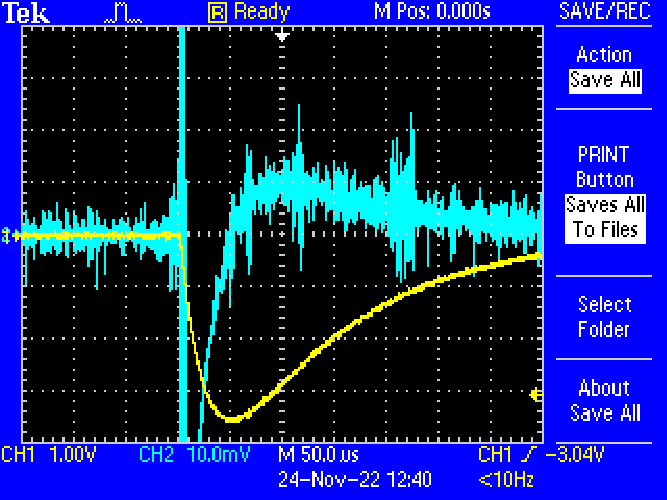
\includegraphics[scale=0.5]{rogowskii-2.pdf}
    \caption{鎖交数が2の時の測定結果}
\end{figure}

\begin{figure}[H]
    \centering
    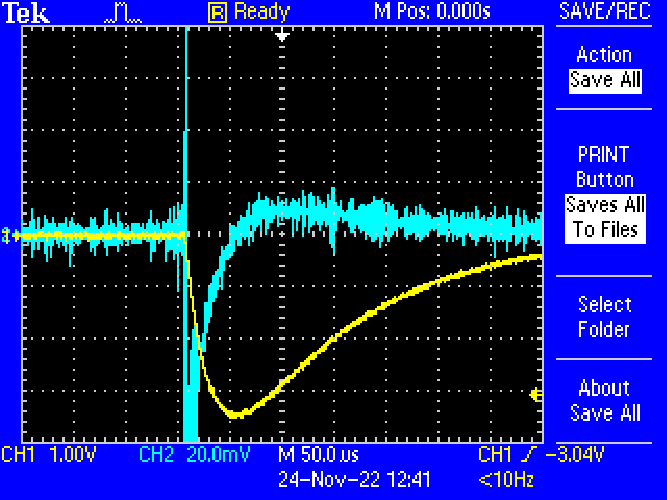
\includegraphics[scale=0.5]{rogowskii-3.pdf}
    \caption{鎖交数が3の時の測定結果}
\end{figure}

\begin{figure}[H]
    \centering
    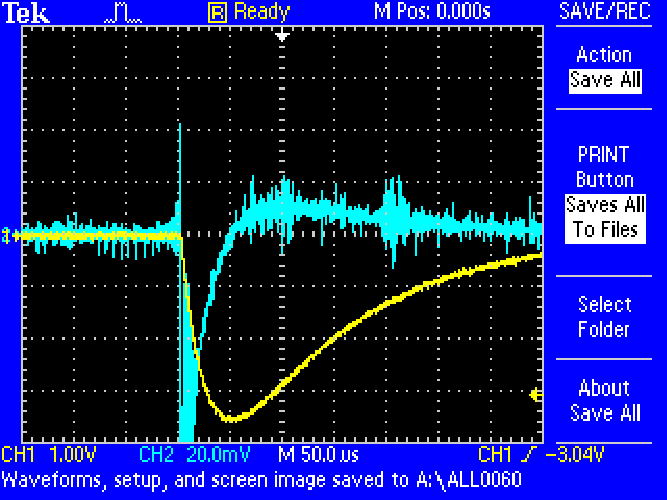
\includegraphics[scale=0.5]{rogowskii-4.pdf}
    \caption{鎖交数が4の時の測定結果}
\end{figure}

\begin{figure}[H]
    \centering
    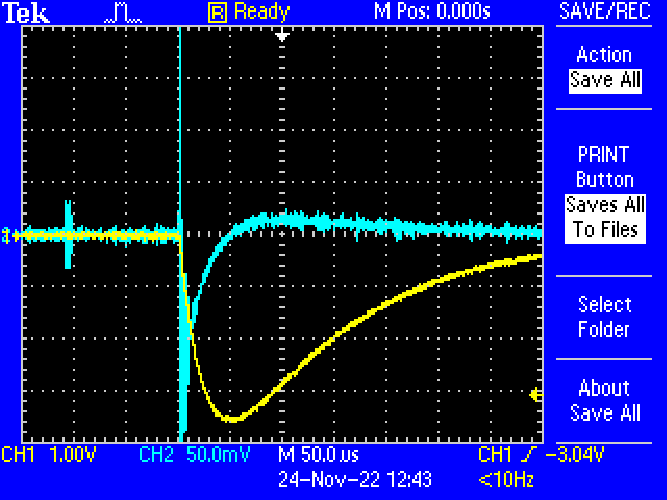
\includegraphics[scale=0.5]{rogowskii-5.pdf}
    \caption{鎖交数が5の時の測定結果}
\end{figure}

\begin{table}[!ht]
    \centering
    \caption{ロゴスキーコイルの出力$V_e$の積分結果}
    \begin{tabular}{c|c}
    \hline
        鎖交回数 & $\int_{0}^{t}V_e(t)dt\,[\si{\mu \volt}]$ \\ \hline
        1 & 0.523 \\ 
        2 & 1.09 \\ 
        3 & 1.53 \\ 
        4 & 1.70 \\ 
        5 & 2.39 \\ \hline
    \end{tabular}
\end{table}
% % !TEX root = main.tex

%%%%%%%%%%%%%%%%%%%%%%%%%%%%%%%%%%%%%%%%%%%%%%%%%%%%%%%%%%%%%%%%%%%%%%%%%%%%%%%%%%%%%%%%%%%%%%%%
\section{データ解析と考察}
%%%%%%%%%%%%%%%%%%%%%%%%%%%%%%%%%%%%%%%%%%%%%%%%%%%%%%%%%%%%%%%%%%%%%%%%%%%%%%%%%%%%%%%%%%%%%%%%
\begin{enumerate}
    \item 実験課題1で得られた結果から,ソレノイド中心軸上の軸方向磁束密度分布
    $B_z(z)$を算出せよ.ただし,導出過程も示すこと.
    \begin{description}
        \item[] 各$z$座標における磁気プローブの出力$V_{co}$を積分し,
        $\int_{0}^{t} V_{co}(t)dt$を算出する.その後,ソレノイド中心軸上の軸方向磁束密度分
        布$B_z(z)$を以下の式で求め,算出結果を有効数字3桁で表3に示す。
        $$
        B=-\frac{1}{NS}\int_{0}^{t} V_{co}(t)dt
        $$
        ただし、各パラメータは次のようになる.
        $$
        N=33\,[回],S=\pi r^2=\pi \times 0.00275^2 \simeq 2.38\times 10^{-5}\,[\si{m^2}]
        $$

        %chart
    \end{description}

    \item ソレノイド中心軸上の軸方向磁束密度分布$B_z(z)$をビオ・サバールの法則
    を用いて計算せよ.ただし,ビオ・サバールの法則を明確に示し,そこからソレノイド
    中心軸上の磁束密度を求める導出過程も詳細に記述すること.
    \begin{description}
        \item[] ビオ・サバールの法則より以下の式が成り立つ.
        $$
        \vec{dB}=\frac{\mu_0 I}{4\pi}\frac{\vec{dl}\times\vec{r}}{|\vec{r}|^3}
        $$
        ここで,図1のような有限長ソレノイドについて考えると,単位長さあたりの
        電流は$nIdz$であるから,ビオ・サバールの法則より,
        $$
        dB=\frac{\mu_0}{4\pi}\frac{nIdzdl\sin\theta}{r^2}=-\frac{\mu_0}{4\pi}\frac{nI\sin\theta}{a}dld\theta
        $$
        となる。ここで$\int_{c}dl=2\pi ab$であり,
        $d\theta$を$\theta_1 \rightarrow \theta_2$で積分すると,
        以下の式が成り立つ.
        $$
        B=\frac{\mu_0 NI}{2}(\cos\theta_2 - \cos\theta_1)
        $$
        したがって,ソレノイド中心軸上の磁束密度は以下の式で求められ,
        その算出結果を有効数字3桁で表4に示す.
        $$
        B_z=\frac{\mu_0 NI}{2}\{\frac{z}{\sqrt[]{a^2+z^2}}+\frac{b-z}{\sqrt[]{a^2+(z-b)^2}}\}
        $$
        ただし,各パラメータは,
        $$
        N=33,\mu_0=1.257\times 10^{-6}\,[\si{H/m}],a=0.0465\,[\si{m}],b=0.250\,[\si{m}]
        $$
        となり,電流$I$は$R=10.6\,[\si{\Omega}]$に関して,$I=\frac{V_R}{R}$で求める.
        %chart
    \end{description}
    
    \item 設問(1)および(2)で得られた結果をグラフに重ね書きしなさい.そして,
    貴方のプローブ測定精度を有効数字2桁で示せ.
    \begin{description}
        \item[] 設問(1)および(2)で得られた結果を重ね書きしたグラフを図 に示す.
        プローブ測定精度を以下の式で求め,その算出結果を有効数字2桁で表5に示す.
        $$
        \frac{\delta B}{B}=\frac{実験値-理論値}{理論値}
        $$
    \end{description}

    \item 実験課題2において,抵抗$R$の両端の電圧波形$V_R$から閉ループ回路に
    流れるパルス電流の最大値を求めよ.導出過程も示すこと.
    \begin{description}
        \item[] 各鎖交数における電圧波形$V_R$におけるピーク電圧$V_{Rmax}$を
        読み取ることで,閉ループ回路に流れるパルス電流の最大値$IR$は以下の式で
        算出される.
        $$
        I_R=\frac{V_{Rmax}}{R}
        $$
        この算出結果を有効数字3桁で表6に示す.ただし,$R= 10.5\,[\Omega]$
        である.表6より,パルス電流の最大値の最確値は次のように求められる.
        $$
        I_{RS}=
        $$
    \end{description}
    
    \item 実験課題2において,ロゴスキーコイルの出力$V_e$から閉ループ回路に
    流れるパルス電流の最大値を求めよ.導出過程も示すこと.
    \begin{description}
        \item[] 閉ループ回路に流れるパルス電流は以下の式で算出される.
        $$
        i_e=-\frac{l}{\mu_0 NS}\int_{0}^{t}V_e(t)dt
        $$
        この算出結果を表7に示す.ただし,各パラメータは次のようになる.
        $$
        \mu_0=1.257\times 10^{-6}\,[\si{H/m}],N=219,S=\pi\times 0.11875^2\simeq 0.04430\,[\si{m^2}],l=2\pi\times 0.11875\simeq 0.7461\,[\si{m}]
        $$
        表7より,パルス電流の最大値の最確値は次のように求められる.
        $$
        I_{es}=
        $$
    \end{description}
    
    \item 実験課題2において,閉ループ回路に流れるパルス電流の最大値を,
    閉ループ回路の回路方程式を解くことによって求めよ.導出過程も示すこと.
    \begin{description}
        \item[] 本実験で用いた閉ループ回路の回路方程式は以下のように表される.
        $$
        L\frac{di}{dt}+Ri+\frac{1}{C}\int idt=V
        $$
        ここで,臨界制動波形であることから、$R^2=\frac{4L}{C}$を満たすので,
        閉ループ回路に流れるパルス電流は以下の式で表される.
        $$
        i=e^{-\frac{R}{2L}t}(C_1+C_2t)
        $$
        ここで,初期条件より$t=0$において,$i=0$,$L\frac{di}{dt}=V$
        であるので,$C_1=0$,$C_2=\frac{V}{L}$となる.
        したがって,閉ループ回路に流れるパルス電流は以下の式で算出される.
        $$
        i=\frac{V}{L}te^{-\frac{R}{2L}t}
        $$
        ここで,パルス電流が最大値を取る時の$t$,充電電圧$V$,ソレノイドコイル
        のインダクタンス$L$,可変抵抗$R$の値は,
        $$
        t=
        $$
        となるので,パルス電流の最大値は次のように求められる.
        $$
        i=\frac{V}{L}te^{-\frac{R}{2L}t}=
        $$
    \end{description}
    
    \item 設問(4)~(6)で求めた値を比較し,その妥当性を検討せよ.
    \begin{description}
        \item[] 
    \end{description}

    \item 実験課題2において,パルス電流が流れている閉ループとロゴスキーコイル
    の間に存在する相互インダクタンス$M$は,式42で与えられる関係を持つ.
    実際に得られた実験値から,相互インダクタンス$M$を求めよ.導出過程も明記すること.
    \begin{description}
        \item[] 42式より$V_e=M\frac{di}{dt}$が成り立ち,この両辺を$t$
        で積分すると以下の式が成り立つ.
        $$
        \int_{0}^{t}V_e(t)dt=Mi
        $$
    \end{description}
\end{enumerate}
% % !TEX root = main.tex

%%%%%%%%%%%%%%%%%%%%%%%%%%%%%%%%%%%%%%%%%%%%%%%%%%%%%%%%%%%%%%%%%%%%%%%%%%%%%%%%%%%%%%%%%%%%%%%%
\section{演習課題}
%%%%%%%%%%%%%%%%%%%%%%%%%%%%%%%%%%%%%%%%%%%%%%%%%%%%%%%%%%%%%%%%%%%%%%%%%%%%%%%%%%%%%%%%%%%%%%%%

\subsection{$f=f_L,f_H$の場合}
\begin{figure}[H]
    \begin{center}
        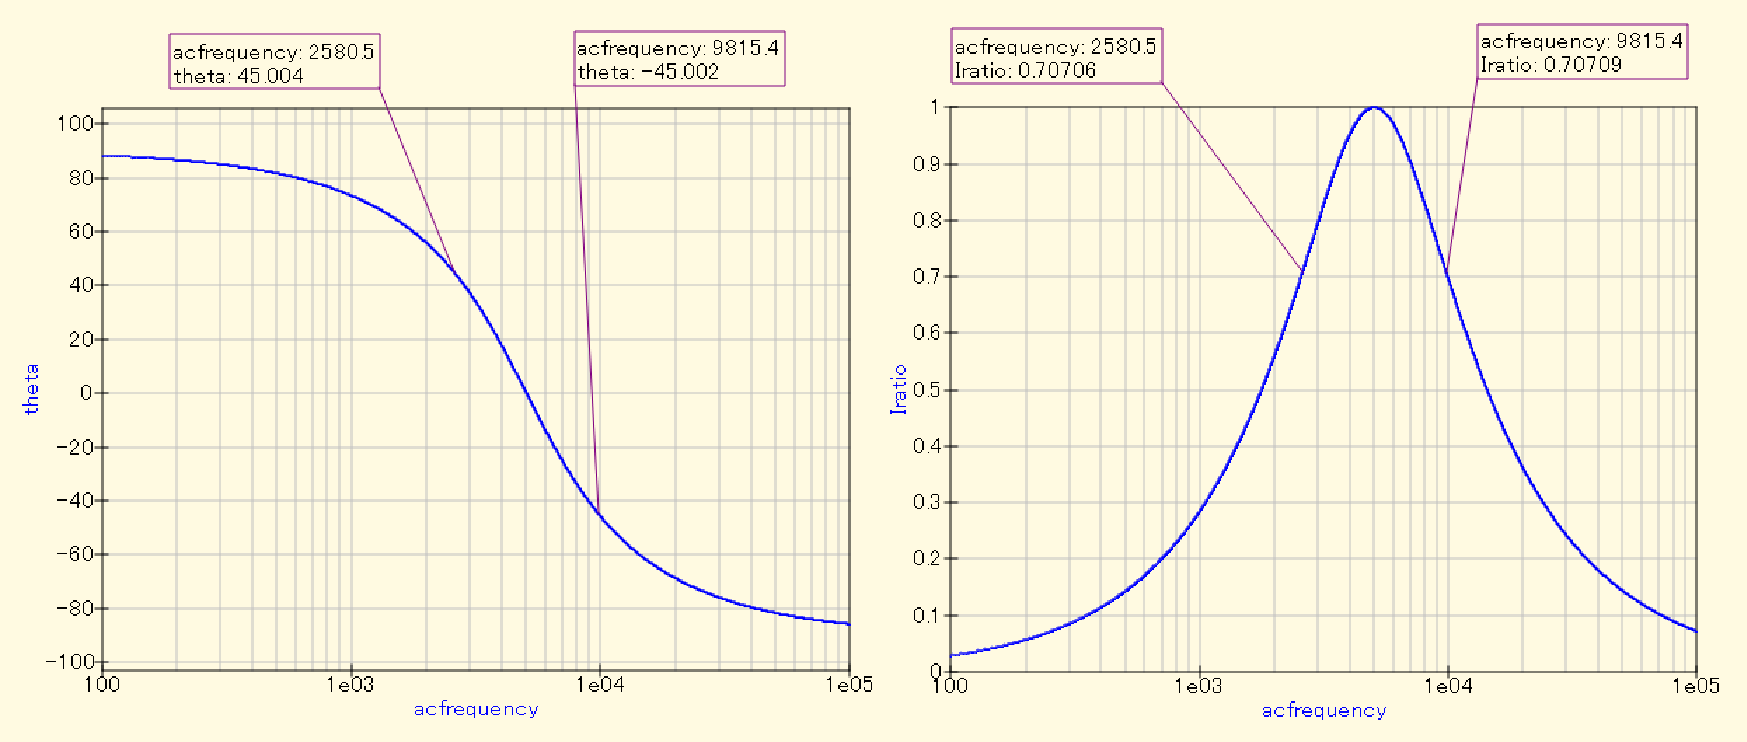
\includegraphics[scale=0.5]{45.pdf}
        \caption{理想コイルにおける$f=f_L,f_H$の場合のインピーダンス偏角の周波数特性}
    \end{center}
\end{figure}

$f=f_L,f_H$においてインピーダンス偏角はそれぞれarg\,$Z=45^\circ,-45^\circ$となる.

\subsection{理想コイルとそうでない場合の比較}
\begin{figure}[H]
    \begin{center}
        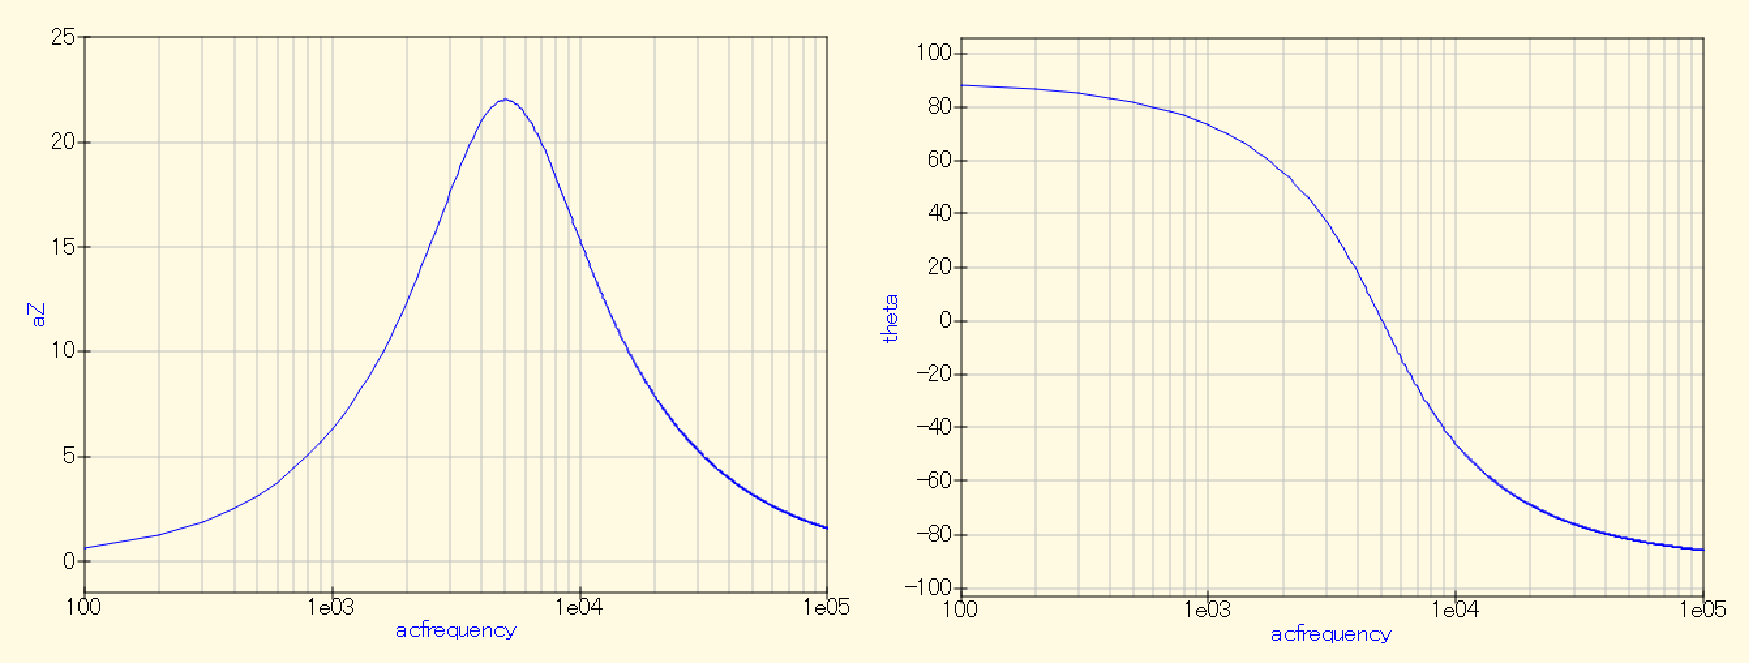
\includegraphics[scale=0.5]{ideal.pdf}
        \caption{理想コイルにおけるインピーダンス周波数特性およびインピーダンス偏角の周波数特性}
    \end{center}
\end{figure}

\begin{figure}[H]
    \begin{center}
        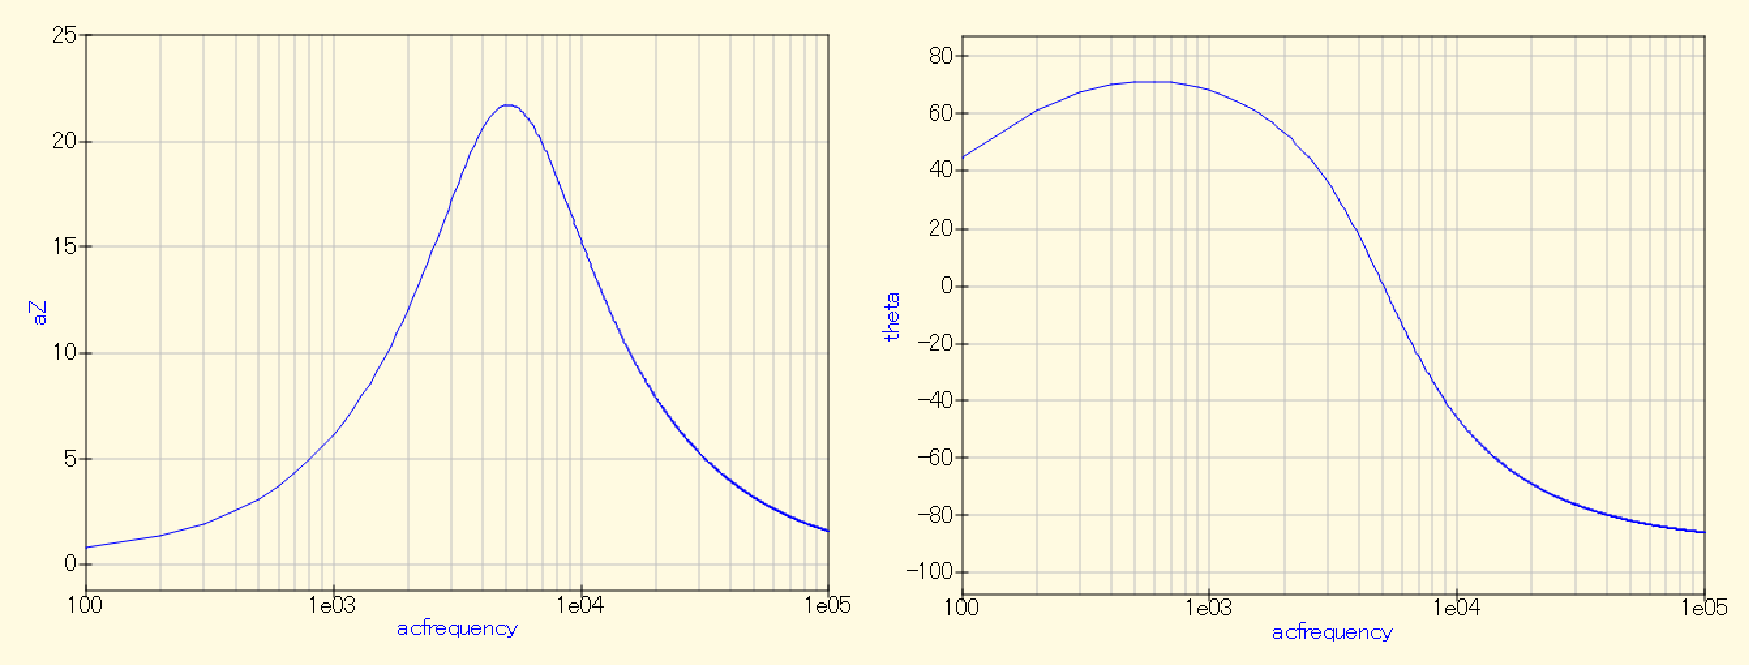
\includegraphics[scale=0.5]{not_ideal.pdf}
        \caption{理想でないコイルにおけるインピーダンス周波数特性およびインピーダンス偏角の周波数特性}
    \end{center}
\end{figure}

インピーダンスの大きさの周波数特性では顕著な差は見られないが,
インピーダンスの偏角の周波数特性では顕著な差が見られる.
% \input{section7.tex}

%%%%%%%%%% 参考文献 %%%%%%%%%%%%%%%%%%%%%%%%%%%%%%%%%%%%%%%%%%%%%%%%%%%%%%%%%%%%%%%%%%%%%%%%%%%%%%

% !TEX root = main.tex

%%%%%%%%%% 参考文献 %%%%%%%%%%%%%%%%%%%%%%%%%%%%%%%%%%%%%%%%%%%%%%%%%%%
\begin{thebibliography}{99}
    \newcounter{num}
    \setcounter{num}{2}
    \bibitem{電子システム工学基礎実験テキスト}
\end{thebibliography}

\end{document}